% Preamble
\documentclass [11pt]{article}

\usepackage{setspace}
\usepackage{amssymb}
\usepackage{amsmath}
\usepackage{amsfonts}
\usepackage{amssymb}
\usepackage{setspace}
\usepackage{amsthm}
\usepackage{textcomp}
\usepackage{graphicx}
\usepackage{url}
\usepackage{color}
\usepackage[dvipsnames]{xcolor}
\definecolor{cuteBlue}{rgb}{0.258, 0.387, 0.574}
\definecolor{cuteGreen}{rgb}{0, 0.3, 0}
\usepackage{cancel}
\usepackage{comment}
\usepackage[framemethod=TikZ]{mdframed}
\usepackage{enumitem}
\usepackage{wasysym}
\usepackage{listings}
\usepackage{float}
\usepackage{booktabs}
\usepackage{fixltx2e}
\usepackage{threeparttable}
\usepackage{titling}
\usepackage{zref-base}
\usepackage{makecell}
\usepackage{array}
\usepackage{hhline}
\usepackage{titlesec}

% To make jumping between equation, figure, citation references easier
\usepackage[colorlinks=true, urlcolor=cuteBlue, citecolor=cuteGreen, linkcolor=black]{hyperref}
%\usepackage[urlcolor=blue, hyperfootnotes=false, hyperfigures=false, hyperindex=false, linkcolor=black]{hyperref}
%\usepackage[colorlinks=true, urlcolor=blue, hyperfootnotes=false, hyperfigures=false, hyperindex=false, linkcolor=red]{hyperref}

% To make caption labels (i.e. Figure 1, Figure 2...) bold and make all caption text small
\usepackage[labelfont=bf, font=small]{caption}
%\usepackage[labelfont=bf, font=small, margin=1cm]{caption}

% To use \nicefrac
\usepackage{units, xfrac}

% For strike-out text during editing
\usepackage[normalem]{ulem}

%Latin accents
\usepackage[utf8]{inputenc}

%subfigures
\usepackage{caption}
\usepackage{subcaption}
% Margins and spacings
\setlength{\evensidemargin}{0.0cm}
\setlength{\oddsidemargin}{0.0cm}
\setlength{\topmargin}{-1.0cm}
\setlength{\textwidth}{17cm}
\setlength{\textheight}{22cm}
\setlength{\parskip}{2.5mm}
\reversemarginpar
\marginparsep  0.1in
\marginparwidth 0.7in

% Give more spacing in equation arrays
\setlength{\jot}{10pt}

% Allow page breaks in multiline equations
\allowdisplaybreaks

% Set up title spacing so we don't waste so much space
\setlength{\droptitle}{-8em}
\date{\vspace{-5em}}  % No date will appear in title.

% Spacing between section headings and text
\titlespacing\section{0pt}{12pt plus 4pt minus 2pt}{-2pt plus 2pt minus 2pt}
\titlespacing\subsection{0pt}{12pt plus 4pt minus 2pt}{-2pt plus 2pt minus 2pt}
\titlespacing\subsubsection{0pt}{12pt plus 4pt minus 2pt}{-2pt plus 2pt minus 2pt}

% Set up problem structure
\newtheoremstyle{break}% name
  {}%         Space above, empty = `usual value'
  {2em}%         Space below
  {}%         Body font
  {}%         Indent amount (empty = no indent, \parindent = para indent)
  {\bfseries}% Thm head font
  {.}%        Punctuation after thm head
  {\newline}% Space after thm head: \newline = linebreak
  {}%         Thm head spec

% Problems and solutions with counter
\newcounter{solution}
\renewcommand{\thesolution}{\arabic{solution}}


% %%%%%%%%%%%%%%%%%%%%%%%%%%%%%%%%%%%%%%%%%%%%%%%%%%%%%%%%%%%%%%%%%%%
% Set up boxes for solutions
% %%%%%%%%%%%%%%%%%%%%%%%%%%%%%%%%%%%%%%%%%%%%%%%%%%%%%%%%%%%%%%%%%%%
%% setup the solution environment
\mdfdefinestyle{solution}{%
    outerlinewidth=2pt,
    bottomline=false,
    leftline=false,rightline=false,
    topline=false,
    font=\small,%
    backgroundcolor=gray!20,%
    skipabove=-5em,
    skipbelow=\baselineskip,
    roundcorner=10pt,%
    innertopmargin=1em,%
    innerbottommargin=1em,%
    splittopskip=1em,%
    splitbottomskip=1em,%
    frametitle=\mbox{},
}
\newmdenv[%
    style=solution,
    settings={\global\refstepcounter{solution}},
    frametitlefont={\bfseries Solution~\thesolution\quad},
]{solution}

%% Shaded box
\newmdenv[style=solution]{shaded}

%% setup the solution environment
\mdfdefinestyle{unshaded}{%
    outerlinewidth=1pt,
    bottomline=true,
    leftline=true,rightline=true,
    topline=true,
    font=\small,%
    backgroundcolor=white,%
    skipabove=-5em,
    skipbelow=\baselineskip,
    roundcorner=10pt,%
    innertopmargin=1em,%
    innerbottommargin=1em,%
    splittopskip=1em,%
    splitbottomskip=1em,%
    frametitle=\mbox{},
}

%% Unshaded box
\newmdenv[style=unshaded]{unshaded}
% %%%%%%%%%%%%%%%%%%%%%%%%%%%%%%%%%%%%%%%%%%%%%%%%%%%%%%%%%%%%%%%%%%%
% %%%%%%%%%%%%%%%%%%%%%%%%%%%%%%%%%%%%%%%%%%%%%%%%%%%%%%%%%%%%%%%%%%%


% Convenient micron symbol
\newcommand{\micron}{{\textmu}m}

\theoremstyle{break}
\newtheorem{problem}{Problem}

%% \theoremstyle{break2}
%% \newtheorem{solution}{Solution}
%% \numberwithin{solution}{section}

% No excess spacing for lists
\setlist{itemsep=0pt, topsep=0pt}

% Allow paragraph indentations in lists
\setitemize{listparindent=\parindent}
\setenumerate{listparindent=\parindent}

% Column type for tables with nice spacing
\newcolumntype{M}[1]{>{\centering\arraybackslash}m{#1}}
\newcolumntype{N}{@{}m{0pt}@{}}

% %%%%%%%%%%%%%%%%%%%%%%%%%%%%%%%%%%%%%%%%%%%%%%%%%%%%%%%%%%%%%%%%%%%
% Settings for display of code
% %%%%%%%%%%%%%%%%%%%%%%%%%%%%%%%%%%%%%%%%%%%%%%%%%%%%%%%%%%%%%%%%%%%
\definecolor{mygreen}{rgb}{0,0.6,0}
\definecolor{mygray}{rgb}{0.5,0.5,0.5}
\definecolor{mymauve}{rgb}{0.58,0,0.82}

\lstset{ %
  backgroundcolor=\color{gray!20},   % choose the background color; you must add \usepackage{color} or \usepackage{xcolor}
  basicstyle=\footnotesize\ttfamily, % the size of the fonts that are used for the code
  breakatwhitespace=false,         % sets if automatic breaks should only happen at whitespace
  breaklines=true,                 % sets automatic line breaking
  captionpos=b,                    % sets the caption-position to bottom
  commentstyle=\color{mygreen},    % comment style
  deletekeywords={...},            % if you want to delete keywords from the given language
  escapeinside={\%*}{*)},          % if you want to add LaTeX within your code
  extendedchars=true,              % lets you use non-ASCII characters; for 8-bits encodings only, does not work with UTF-8
  frame=single,                    % adds a frame around the code
  keepspaces=true,                 % keeps spaces in text, useful for keeping indentation of code (possibly needs columns=flexible)
  keywordstyle=\color{blue},       % keyword style
  morekeywords={*,...},            % if you want to add more keywords to the set
  numbers=left,                    % where to put the line-numbers; possible values are (none, left, right)
  numbersep=5pt,                   % how far the line-numbers are from the code
  numberstyle=\tiny\color{mygray}, % the style that is used for the line-numbers
  rulecolor=\color{black},         % if not set, the frame-color may be changed on line-breaks within not-black text (e.g. comments (green here))
  showspaces=false,                % show spaces everywhere adding particular underscores; it overrides 'showstringspaces'
  showstringspaces=false,          % underline spaces within strings only
  showtabs=false,                  % show tabs within strings adding particular underscores
  stepnumber=2,                    % the step between two line-numbers. If it's 1, each line will be numbered
  stringstyle=\color{mymauve},     % string literal style
  tabsize=2,                       % sets default tabsize to 2 spaces
  title=\lstname,                   % show the filename of files included with \lstinputlisting; also try caption instead of title
  xleftmargin=2em,                 % Indent the listings
  belowskip=-2em                      % No extra space below listing
}

%% Code below removes line numbering for listings that have less than 12 lines
\makeatletter
\newcounter{mylstlisting}
\newcounter{mylstlines}
\lst@AddToHook{PreSet}{%
  \stepcounter{mylstlisting}%
  \ifnum\mylstlines<12\relax
    \lstset{numbers=none}
  \else
    \lstset{numbers=left}
  \fi
  \setcounter{mylstlines}{0}%
}
\lst@AddToHook{EveryPar}{%
  \stepcounter{mylstlines}%
}
\lst@AddToHook{ExitVars}{%
  \begingroup
    \zref@wrapper@immediate{%
      \zref@setcurrent{default}{\the\value{mylstlines}}%
      \zref@labelbyprops{mylstlines\the\value{mylstlisting}}{default}%
    }%
  \endgroup
}

% \mylstlines print number of lines inside listing caption
\newcommand*{\mylstlines}{%
  \zref@extractdefault{mylstlines\the\value{mylstlisting}}{default}{0}%
}
\makeatother

% %%%%%%%%%%%%%%%%%%%%%%%%%%%%%%%%%%%%%%%%%%%%%%%%%%%%%%%%%%%%%%%%%%%
% %%%%%%%%%%%%%%%%%%%%%%%%%%%%%%%%%%%%%%%%%%%%%%%%%%%%%%%%%%%%%%%%%%%

%Add a printed pdf page
\usepackage{pdfpages}
\usepackage{mathtools}
\usepackage{wrapfig}

% Add author affiliations
\usepackage{authblk}


% import macro for the figures path % this will not be synchronized to the
% GitHub repository since each collaborator will adapt it to his/her own
% directory structure
\input{graphicspath.tex}

%%%%%%%%%%%%%%%%%%%%%%%%%%%%%%%%%%%%%%%%%%%%%%%%%%%%
%% Begin packages
%%%%%%%%%%%%%%%%%%%%%%%%%%%%%%%%%%%%%%%%%%%%%%%%%%%%
% Commenting
\newcommand{\mrm}[1]{\textcolor{ForestGreen}{(MR:~#1)}} % Commenting
\newcommand{\rp}[1]{\textcolor{red}{(RP:~#1)}} % Commenting

% To bold the first sentence of every figure caption
\newcommand{\captionStroke}[1]{\textbf{#1}}

% To define more useful LaTeX commands
\usepackage{xparse}

% Equation referencing
\newcommand{\eref}[1]{Eq.~\ref{#1}}
% \DeclareDocumentCommand \eref{oooo}{\IfNoValueTF{#2}{Eq.~(\ref{#1})}
% {\IfNoValueTF{#3}{Eqs.~(\ref{#1}) and (\ref{#2})}
% {\IfNoValueTF{#4} {Eqs.~(\ref{#1})-(\ref{#3})}
% {Eqs.~(\ref{#1})-(\ref{#4})}}}}
%
% Figure referencing
\newcommand{\fref}[1]{Fig.~\ref{#1}}
% \DeclareDocumentCommand \fref{ooo}
% {\IfNoValueTF{#2}{Fig.~\ref{#1}}{\IfNoValueTF{#3}{Figs.~\ref{#1} and
% \ref{#2}}{Figs.~\ref{#1}-\ref{#3}}}}

% Letters for figure sub-parts
\newcommand{\letter}[1]{#1} % For main text. Ex: As shown in Fig. 12A
\newcommand{\letterParen}[1]{(#1)} % For captions. Ex: (A) Low limit and (B) high limit

%%%%%%%%%%%%%%%%%%%%%%%%%%%%%%%%%%%%%%%%%%%%%%%%%%%%
% Personalized functions
%%%%%%%%%%%%%%%%%%%%%%%%%%%%%%%%%%%%%%%%%%%%%%%%%%%%
\newcommand{\kpon}{k^{(p)}_{\text{on}}}
\newcommand{\kpoff}{k^{(p)}_{\text{off}}}
\newcommand{\kron}{k^{(r)}_{\text{on}}}
\newcommand{\kroff}{k^{(r)}_{\text{off}}}
\newcommand{\gm}{\gamma _m}
\newcommand{\gp}{\gamma _p}
\newcommand{\ee}[1]{\left\langle #1 \right\rangle}
\newcommand{\bb}[1]{\mathbf{#1}}
\newcommand{\dt}[1]{{\partial{#1} \over \partial t}}
\newcommand{\PP}{\bb{P}}
\newcommand{\Km}{\bb{K}}
\newcommand{\Rm}{\bb{R}_m}
\newcommand{\Gm}{\bb{\Gamma}_m}
\newcommand{\Rp}{\bb{R}_p}
\newcommand{\Gp}{\bb{\Gamma}_p}

%%%%%%%%%%%%%%%%%%%%%%%%%%%%%%%%%%%%%%%%%%%%%%%%%%%%
%% Begin document
%%%%%%%%%%%%%%%%%%%%%%%%%%%%%%%%%%%%%%%%%%%%%%%%%%%%
\title{\textbf{First-principles prediction of the information processing
capacity of a simple genetic circuit}}
\author{Manuel Razo-Mejia and Rob Phillips}
\date{\today}

\begin{document}
\maketitle
	% As living organisms thrive in the environment, they are faced with constant
changes in their surroundings. From abiotic conditions to biological
interactions, living organisms at all organization levels sense and respond to
external signals. At the molecular level, where signal transduction components
exist, there are physical constraints on the accuracy and precision of these
responses given by the intrinsic stochastic fluctuations  \cite{Nemenman2010}.
This means that two genetically identical cells exposed to the same stimulus
will not have an identical response \cite{Eldar2010}.

The implications of this biological noise is that cells do not have an infinite
resolution to distinguish signals and as a consequence there is a one-to-many
mapping between inputs and outputs. The question then becomes how to analyze
this probabilistic rather than deterministic relationship between inputs and
outputs? The abstract answer to this question was worked out in 1948 by Claude
Shannon who, in his seminal work, founded the field of information theory
\cite{Shannon1948}. Shannon developed a general framework for how to analyze
information transmission through noisy communication channels. In his work,
Shannon showed that the only quantity that satisfies simple conditions of what a
metric for information should be, was of the same functional form as the
thermodynamic entropy -- thereby naming it the same \cite{MacKay2003}. He also
gave a definition, based on this information entropy, for the relationship
between inputs and outputs known as the mutual information (see Appendix XX for
details on these metrics). \mrm{This would be a useful appendix regardless of
the type of journal.}

It is natural to think that under certain scenarios living organisms that can
better resolve signals might have an evolutionary advantage, making it more
likely that their offspring will have a higher fitness value \cite{Taylor2007a}.
In recent years there has been a growing interest in understanding the
theoretical limits on cellular information processing \cite{Bialek2005,
Gregor2007}, and in quantifying how close evolution has pushed cellular
signaling pathways to these theoretical limits \cite{Tkacik2008, Dubuis2013,
Petkova2016}. While these studies have treated the signaling pathway as a
``black box'' explicitly ignoring all the molecular interactions taking place in
them, other studies have explored the role that molecular players and regulatory
architectures have on these information processing tasks \cite{Rieckh2014,
Ziv2007, Voliotis2014, Tostevin2009, Tkacik2011, Tkacik2008a, Tabbaa2014}. These
studies on the other hand have assumed a specific functional form for the noise
level rather than deriving it from a discrete stochastic model \mrm{double check
this statement!}. This has the limitation that at small numbers the functional
form of the noise might not be well approximated by a continuous function.

On the other hand, over the last decade the dialogue between theory and
experiments in gene regulation has led to predictive power not only over the
mean, but the noise in gene expression as a function of relevant parameters such
as regulatory protein copy numbers, affinity of these proteins to the DNA
promoter, as well as the extracellular concentrations of inducer
molecules \cite{Garcia2011c, Jones2014a, Brewster2014, Razo-Mejia2018} \mrm{Too
self referential so far. Include Ido, maybe Al Sanchez. It must be
experiment-theory contrasting though!}. These models based on equilibrium and
non-equilibrium statistical physics have reached a predictive accuracy level
such that for simple cases it is now possible to design input-output functions
\cite{Brewster2012, Barnes2018}. This opens the possibility to exploit the
advancements on these predictive models to tackle the question of how much
information can genetic circuits process.

In this work we follow the same philosophy of theory-experiment dialogue to
predict from first principles the effect that biophysical parameters such as
transcription factor copy number and protein-DNA affinity have on the
information processing capacity of a simple genetic circuit. Specifically we use
a master-equation-based model to construct the protein copy number distribution
(output) as a function of an extracellular inducer concentration (input) for
different combinations of transcription factor copy numbers and binding sites.
We then compute the channel capacity, i.e. the maximum information that can be
processed by this gene regulatory architecture. All parameters used for our
model were inferred from a series of studies that span several experimental
techniques \cite{Garcia2011c, Brewster2012, Jones2014a, Brewster2014,
Razo-Mejia2018} \mrm{see Appendix XX Parameter inference}, allowing us to
perform zero-parameter fit predictions of this non-trivial quantity.
\mrm{Aztec pyramid reference}

These predictions are then contrasted with experimental data, where the channel
capacity is inferred from single-cell fluorescence distributions taken at
different concentrations of inducer for cells with previously characterized
biophysical parameters \cite{Garcia2011c, Razo-Mejia2018}. We find that our
parameter free predictions closely match the experiments.
\mrm{need to work on a more impactful last paragraph.}

	% \section{Models}

\textcolor{blue}{Introduce Jane's paper as a means of mRNA variability}


\begin{figure}[h!]
	\centering \includegraphics[scale=0.1]{Figure2.jpg} \caption{Channel capacity of the Lac repressor. Experimental data with \textbf{theory perfectly overlaid on top}, omg bbq roflcopter!}
	\label{figChannelCapacity}
\end{figure}

\begin{figure}[h!]
	\centering \includegraphics[scale=0.2]{Figure3v2.jpg} \caption{Experimental results of gene expression overlaid with theoretical prediction. \talComment{Show all results for O2, say that other plots are in SI}}
	\label{figFullProfile}
\end{figure}

\talComment{Potential other figures:
	\begin{itemize}
		\item Varying cross all $R$ and $k_{off}$ values, what is the maximal channel capacity you can achieve?
		\item Potentially look at Mitch Lewis's strains which will have different $K_{DNA}$ or $K_{A}$ and $K_{I}$ parameters and redo the analysis there, showing that the theory is amazingly good!
	\end{itemize}
	}

\talComment{Other things that would be very interesting to explore:
\begin{itemize}
	\item Explore the channel capacity analytically in the limit of small noise (discuss whether this is a valid assumption from our data)
	\item Be theorists, and consider how other variables affect the channel capacity. For example, the (active) repressor-DNA binding energy, or $K_A/K_I$, or the rates in the problem. Would be really cool to basically look at the effects of all of the variables that we have on channel capacity, and consider which yield the coolest results.
\end{itemize}
}
	% \section{Results}

To test our theory, we measured the gene expression distribution for a synthetic
circuit. \fref[figFullProfile] shows the data for different O2 strains with
varying numbers of the Lac repressor $R$ spanning two orders of magnitude.
Overlaid on this data is the theory from
\eref[eqGeneExpressionDistributionFastRates].

\begin{figure}[h!]
	\centering \includegraphics[scale=0.16]{Figure3v2.jpg} 
	\caption{\captionStroke{Experimental results of gene expression overlaid with theoretical prediction.} Gene expression is shown for the O2 operator for different repressor copy numbers. The gene expression profiles for the O1 and O3 operators are shown in the Supporting Information.}
	\label{figFullProfile}
\end{figure}

We next computed the channel capacity for the Lac system using
\eref[eqChannelCapacity], as shown in \fref[figChannelCapacity].

\begin{figure}[h!]
	\centering \includegraphics[scale=0.1]{Figure2.jpg} 
	\caption{\captionStroke{Channel capacity of the Lac repressor.} Experimental data and theoretical predictions for the channel capacity of the \textit{lac} system. Data was tuned over several different copy numbers of repressor as well as repressor-DNA binding energies.}
	\label{figChannelCapacity}
\end{figure}
	% \section{Derivation of the two stage promoter equation}

Shahreaei and Swain derive the full analytical protein distribution for a two
stage (i.e. an unregulated promoter) and a three stage (i.e. a promoter that
transitions between active and inactive) promoter. In this section wi will
follow the derivation augmenting the details at each step for clarity.

First let us write the chemical master equation for this system. Let $p$ and $m$
be the protein and mRNA copy numbers, respectively, and $P_{m,p}(t)$ be the
probability of having $m$ mRNA and $p$ proteins at time t. Then we can use the
``spread the butter'' approach to write the discrete difference equation
\begin{equation}
\begin{aligned}
P_{m,p}(t + \Delta t) =
P_{m,p}(t)
+ \overbrace{r_m \Delta t \left[ P_{m-1,p}(t) - P_{m,p}(t) \right]}^\text{mRNA
production}
+ \overbrace{r_p m
\Delta t \left[ P_{m, p-1}(t) - P_{m, p}(t) \right]}^\text{protein
production}\\
+ \underbrace{\gamma_m \Delta t \left[ (m + 1) P_{m+1,p}(t) - m P_{m, p}(t)
\right]}_\text{mRNA degradation}
+ \underbrace{\gamma_p \Delta t \left[ (p + 1) P_{m, p+1}(t) - p P_{m, p}(t)
\right]}_\text{protein degradation},
\end{aligned}
\end{equation}
where $r_m$ and $r_p$ are the mRNA and protein production rates respectively,
$\gamma_m$ and $\gamma_p$ are the mRNA and protein degradation rates
respectively, and $\Delta t$ is a time interval small enough so that only one
event can take place.

We rearrange the terms, divide both sides by $\Delta t$ , obtaining
\begin{equation}
  \begin{aligned}
\frac{P_{m,p}(t + \Delta t) - P_{m,p}(t)}{\Delta t} = r_m \left[ P_{m-1,p}(t) -
P_{m,p}(t) \right] + r_p m \left[ P_{m, p-1}(t) - P_{m, p}(t) \right]\\
+ \gamma_m \left[ (m + 1) P_{m+1,p}(t) - m P_{m, p}(t) \right] + \gamma_p \left[
 (p + 1) P_{m, p+1}(t) - p P_{m, p}(t) \right].
  \end{aligned}
\end{equation}
We now take the limit $\Delta t \rightarrow 0$ to obtain the final form of the
chemical master equation
\begin{equation}
\begin{aligned}
\frac{\partial P_{m,p}}{\partial t} = r_m \left[ P_{m-1,p}(t) - P_{m,p}(t)
\right] + r_p m \left[ P_{m, p-1}(t) - P_{m, p}(t) \right]\\
+ \gamma_m \left[ (m + 1) P_{m+1,p}(t) - m P_{m, p}(t) \right] + \gamma_p \left[
(p + 1) p_{m, p+1}(t) - p p_{m, p}(t) \right].
  \end{aligned}
\end{equation}

Let us now divide by the slowest rate, i.e. $\gamma_r$
\begin{equation}
\begin{aligned}
\frac{1}{\gamma_p} \frac{\partial P_{m,p}}{\partial t} =
\frac{r_m}{\gamma_p} \left[ P_{m-1,p}(t) - P_{m,p}(t) \right]
+ \frac{r_p}{\gamma_p} m  \left[ P_{m, p-1}(t) - P_{m, p}(t) \right]\\
+ \frac{\gamma_m}{\gamma_p} \left[ (m + 1) P_{m+1,p}(t) - m P_{m, p}(t)
\right]
+ \left[ (p + 1) P_{m, p+1}(t) - p P_{m, p}(t) \right].
\end{aligned}
\label{eq_cme_over_gammap}
\end{equation}
We now introduce the following variables:
\begin{align}
  a \equiv \frac{r_m}{\gamma_p}\\
  b \equiv \frac{r_p}{\gamma_m}\\
  \gamma \equiv \frac{\gamma_m}{\gamma_p}\\
  \tau \equiv \gamma_p \cdot t
\end{align}
Substituting these variables into \eref[eq_cme_over_gammap] we obtain
\begin{equation}
\begin{aligned}
\frac{\partial P_{m,p}}{\partial \tau} =
a \left[ P_{m-1,p}(t) - P_{m,p}(t) \right]
+ b \gamma m  \left[ P_{m, p-1}(t) - P_{m, p}(t) \right]\\
+ \gamma \left[ (m + 1) P_{m+1,p}(t) - m P_{m, p}(t) \right]
+ \left[ (p + 1) P_{m, p+1}(t) - p P_{m, p}(t) \right].
\end{aligned}
\label{eq_cme_tau}
\end{equation}
Note that we used $\frac{1}{\gamma_p}\frac{\partial}{\partial t} =
\frac{\partial}{\partial \tau}$.

We now define the generating function
\begin{equation}
F\left[ s, z \right] = \sum_{m=0}^{\infty} \sum_{p=0}^{\infty} s^m z^p P_{m, p},
\end{equation}
where from now on we abbreviate $P_{m, p}(t)$ as $P_{m, p}$. The generating
function will allow us to write a single PDE rather than an infinite system of
PDEs for each mRNA and protein copy number. The generating function time
derivative is given by
\begin{equation}
\frac{\partial F}{\partial \tau} =
\frac{\partial}{\partial \tau} \sum_{m=0}^{\infty} \sum_{p=0}^{\infty} s^m z^p
P_{m, p} =
\sum_{m=0}^{\infty}
\sum_{p=0}^{\infty} s^m z^p \frac{\partial}{\partial \tau} P_{m, p}.
\label{eq_dF_dtau}
\end{equation}
We now substitute \eref[eq_cme_tau] into \eref[eq_dF_dtau]
\begin{equation}
\begin{aligned}
\frac{\partial F}{\partial \tau} =
\sum_{m=0}^{\infty} \sum_{p=0}^{\infty} s^m z^p a \left[ P_{m-1,p}(t) -
P_{m,p}(t) \right]
+ b \gamma m  \left[ P_{m, p-1}(t) - P_{m, p}(t) \right]\\
+ \gamma \left[ (m + 1) P_{m+1,p}(t) - m P_{m, p}(t) \right]
+ \left[ (p + 1) P_{m, p+1}(t) - p P_{m, p}(t) \right].
\end{aligned}
\label{eq_dF_dtau_complete}
\end{equation}

Note that
\begin{equation}
\sum_{m=0}^{\infty} \sum_{p=0}^{\infty} s^m z^p \left( P_{m+k, p} - P_{m, p}
\right) =
\sum_{m=0}^{\infty} \sum_{p=0}^{\infty} s^m z^p P_{m+k, p}
- \sum_{m=0}^{\infty} \sum_{p=0}^{\infty} s^m z^p P_{m, p}.
\end{equation}
We can now factorize $s^{-k}$ from the first term on the left hand side and
redefine the variable to sum over.
\begin{equation}
\sum_{m=0}^{\infty} \sum_{p=0}^{\infty} s^m z^p \left( P_{m+k, p} - P_{m, p}
\right) =
s^{-k} \sum_{(m+k)=0}^{\infty} \sum_{p=0}^{\infty} s^{m+k} z^p P_{m+k, p}
- \sum_{m=0}^{\infty} \sum_{p=0}^{\infty} s^m z^p P_{m, p}.
\end{equation}
But since both sums on the left hand side are taken over the same ranges we can
write it as
\begin{equation}
\sum_{m=0}^{\infty} \sum_{p=0}^{\infty} s^m z^p \left( P_{m+k, p} - P_{m, p}
\right) =
\left( s^{-k} - 1 \right) \sum_{m=0}^{\infty} \sum_{p=0}^{\infty} s^m z^p P_{m,
p}
\end{equation}

With this identity we can rewrite \eref[eq_dF_dtau_complete] as
\begin{equation}
\begin{aligned}
\frac{\partial F}{\partial \tau} =
(s - 1) \sum_{m=0}^{\infty} \sum_{p=0}^{\infty} s^m z^p \left( a P_{m,p} \right)
+ (z - 1) \sum_{m=0}^{\infty} \sum_{p=0}^{\infty} s^m z^p b \gamma m P_{m,p}
\\
+ \left( s^{-1} - 1 \right) \sum_{m=0}^{\infty} \sum_{p=0}^{\infty} s^m z^p
\gamma m P_{m,p}
+ \left( z^{-1} - 1 \right) \sum_{m=0}^{\infty} \sum_{p=0}^{\infty} s^m z^p
\gamma p P_{m,p}.
\end{aligned}
\label{eq_dF_dtau_identity}
\end{equation}

Another useful identity can be derived if we note that
\begin{equation}
\sum_{m=0}^{\infty} \sum_{p=0}^{\infty} s^m z^p m P_{m, p} =
\sum_{m=0}^{\infty} \sum_{p=0}^{\infty} z^p s \frac{\partial s^m}{\partial s}
P_{m, p}.
\end{equation}
But since $z^p$ and $P_{m, p}$ do not depend on $s$ we can write
\begin{equation}
\sum_{m=0}^{\infty} \sum_{p=0}^{\infty} s^m z^p m P_{m, p} =
s \frac{\partial}{\partial s}\left( \sum_{m=0}^{\infty} \sum_{p=0}^{\infty} s^m z^p P_{m, p} \right) =
s \frac{\partial}{\partial s}F.
\end{equation}

Using this identity in \eref[eq_dF_dtau_identity] allow us to remove all the
sums, obtaining a single PDE of the form
\begin{equation}
\frac{\partial F}{\partial \tau} =
(s - 1) a F + (z - 1) b \gamma s \frac{\partial F}{\partial s}
+ \left( s^{-1} - 1 \right) \gamma s \frac{\partial F}{\partial s}
+ \left( z^{-1} - 1 \right) z \frac{\partial F}{\partial Z}.
\end{equation}
Rearranging terms we obtain
\begin{equation}
\frac{\partial F}{\partial \tau} =
a (sF - s)
+ b \gamma \left( z s \frac{\partial F}{\partial s} - s \frac{\partial
F}{\partial s} \right)
+ \gamma \left( \frac{\partial F}{\partial s} - s \frac{\partial F}{\partial s}
\right)
+ \left( \frac{\partial F}{\partial z} - z \frac{\partial F}{\partial z}
\right).
\end{equation}

	% \section{Method of the characteristics}

\manuelComment{based on this video: https://www.youtube.com/watch?v=LpHqrlrU5pM}

The method of the characteristics is a powerful method to solve PDE. This method enable us to solve a wide range of problems including:
\begin{enumerate}
  \item Linear:
  \begin{equation}
  a(x, y) \frac{\partial u}{\partial x}
  + b(x, y) \frac{\partial u}{\partial y}
  + c(x, y) u
  = f(x, y)
  \end{equation}
  \item Semi-linear:
  \begin{equation}
  a(x, y) \frac{\partial u}{\partial x}
  + b(x, y) \frac{\partial u}{\partial y}
  + c(x, y) u
  = f(x, y, u)
  \end{equation}
  \item  Quasi-linear:
  \begin{equation}
  a(x, y) \frac{\partial u}{\partial x}
  + b(x, y) \frac{\partial u}{\partial y}
  = f(x, y, u)
  \end{equation}
\end{enumerate}

In this introduction  we will focus on semi-linear problems that also include
the linear ones. Let us consider a PDE of the form
\begin{equation}
  a(x, y) \frac{\partial u}{\partial x}
  + b(x, y) \frac{\partial u}{\partial y}
  = f(x, y, u),
  \label{eq_semi_linear}
\end{equation}
which is a semi-linear PDE. Semi-linear equations include equations of the form
\begin{equation}
  a(x, y) \frac{\partial u}{\partial x}
  + b(x, y) \frac{\partial u}{\partial y}
  + c(x, y) u
  = g(x, y),
\end{equation}
with $f(x, y, u) = g(x, y) - c(x, y) u$.

This PDE must have an initial condition associated with it. This initial
condition can be of the form
\begin{equation}
  u(x, 0) = u_0(x),
\end{equation}
or
\begin{equation}
  u(0, y) = u_1(x).
\end{equation}
The pair of a PDE like \eref[eq_semi_linear] and an initial condition is
sometimes called a semi-linear Cauchy problem.

Any solution to these Cauchy problems can be represented by a surface $u \equiv
u(x, y)$ in a 3D space as schematically shown in \fref[fig_integral_surface]
\begin{figure}[h!]
	\centering 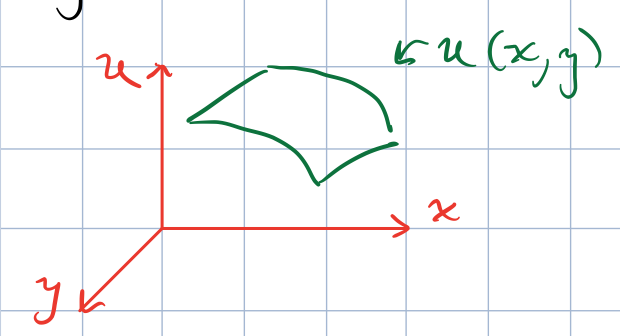
\includegraphics[scale=.75]{fig/fig1_method_characteristics.png}
	\caption{\captionStroke{Schematic integral surface.}}
	\label{fig_integral_surface}
\end{figure}

A surface $u = u(x, y)$ that solves a Cauchy problem is known as an integral
surface since integration is used to solve these problems. We can write down the
equation of this integral surface as
\begin{equation}
  F(x, y, u) \equiv u(x, y) - u = 0.
\end{equation}
Note that the first $u(x, y)$ is a function, while the second $u$ is a
variable. So for example if
\begin{equation}
  u(x, y) = x - y^2,
\end{equation}
then
\begin{equation}
  F(x, y, u) = x - y^2 - u.
\end{equation}

From vector calculus we know that any vector $\mathbf{n}$ normal to the surface $F = 0$ is given by the gradient
\begin{equation}
  \mathbf{n} = \nabla F =
  \frac{\partial u}{\partial x} \mathbf{i}
  + \frac{\partial u}{\partial y} \mathbf{j}
  - \mathbf{k}.
\end{equation}

\fref[fig_normal_vector] shows a schematic representation of this vector. The
vector is represented pointing downwards since $F = u(x, y) - u$.

\begin{figure}[h!]
	\centering 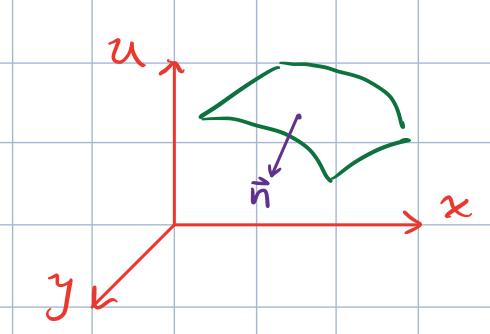
\includegraphics[scale=.75]{fig/fig2_method_characteristics.png}
	\caption{\captionStroke{Schematic integral surface with normal vector.}}
	\label{fig_normal_vector}
\end{figure}

We can rewrite the PDE as a dot product of the form
\begin{equation}
  \left\langle a(x, y), b(x, y), f(x, y, u) \right\rangle \cdot \mathbf{n} = 0.
\end{equation}

This implies that since the dot product is zero, the vector $\left\langle a(x,
y), b(x, y), f(x, y, u) \right\rangle$ must be normal to $\mathbf{n}$. Since we
stated that the vector $\mathbf{n}$ is normal to the surface $F(x, y, u) = 0$,
any vector $\mathbf{v}$ normal to $\mathbf{n}$ must lie in the tangential plane
to $F = 0$ at every point as depicted in \fref[fig_tangential_vector]
\begin{figure}[h!]
	\centering 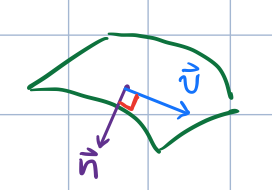
\includegraphics[scale=.75]{fig/fig3_method_characteristics.png}
	\caption{\captionStroke{Schematic integral surface with normal vector
  $\mathbf{n}$ and tangential vector $\mathbf{v}$.}}
	\label{fig_tangential_vector}
\end{figure}

But what do all these details mean? This means that the PDE requires for any
integral surface that solves the equation to be tangential to the vector
\begin{equation}
  \mathbf{v} = a(x,y) \mathbf{i} +
  b(x, y) \mathbf{j} +
  f(x, y, u) \mathbf{k}.
\end{equation}
That is, if we start at some point set by the initial condition and we move in
the direction of the vector $\mathbf{v}$ (which we can determine just by looking
at the PDE) then we move along a curve that lies entirely within the surface
$F = 0$. This curve, depicted in \fref[fig_characteristic_curve] is called a
\textit{characteristic curve}. And by finding the collection of these
characteristic curves we can therefore reconstruct the entire integral surface,
solving therefore the PDE.
\begin{figure}[h!]
	\centering \includegraphics[scale=.75]{fig/fig4_method_characteristics.png}
	\caption{\captionStroke{Schematic of a characteristic curve on an integral
  surface.}}
	\label{fig_characteristic_curve}
\end{figure}

In other words, so far we have shown that given an initial condition
$u(x, 0) = u_0(x)$ as long as we move along the direction given by the vector
$\mathbf{v} = \left\langle a(x,y), b(x,y), f(x,y,u) \right\rangle$ we are
guaranteed to lay on the integral surface. So the process to reconstruct the
entire surface would be to choose a value for $x$, then start at $u_0(x)$ and
move along $\mathbf{v}$; then we would choose a new value of $x$ and repeat the
process. At the end, the union of all these paths along the integral surface
will determine entirely the solution of the PDE. The advantage of the method as
we will show is that walking along the characteristic curve is equivalent to
solving an ODE, which for many cases we know how to do.

We can describe all the points on a characteristic curve by parametrizing
the curve with a vector function
\begin{equation}
  \mathbf{p}(t) = x(t) \mathbf{i} + y(t) \mathbf{j} + u(t) \mathbf{k}.
\end{equation}
Furthermore, we can obtain a vector tangential to this curve $\mathbf{p}(t)$ by
differentiating with respect to the parametrization variable $t$, i.e.
\begin{equation}
  \mathbf{p}'(t) = x'(t) \mathbf{i}+ y'(t) \mathbf{j} + u'(t) \mathbf{k}.
\end{equation}

Since the curve $\mathbf{p}(t)$ lays on the integral surface $F = 0$, and
$\mathbf{p}'(t)$ is tangential to this curve, that means that $\mathbf{p}'(t)$
also lies on the surface.

We stated earlier that if we move along the direction of $\mathbf{v}$ we will
reconstruct the path of the characteristic curve which we now parametrized as
$\mathbf{p}(t)$. That implies that $\mathbf{v}$ and $\mathbf{p}'(t)$ must be
pointing in the same direction, i.e.
\begin{equation}
  \mathbf{p}'(t) = \lambda \mathbf{v},
\end{equation}
where $lambda$ is a scalar. This can also be written as
\begin{equation}
  x'(t)\mathbf{i} + y'(t)\mathbf{j} + u'(t)\mathbf{k} =
  \lambda a(x,y) + \lambda b(x,y) + \lambda f(x,y,u).
\end{equation}
in other words
\begin{align}
  x'(t) = \lambda a(x,y),\\
  y'(t) = \lambda b(x,y), \\
  u'(t) = \lambda f(x,y,u).
\end{align}
We can now solve for $\lambda$ and equate all of the solutions, obtaining
\begin{equation}
  {{dx \over dt} \over a(x,y)}} =
  {{dy \over dt} \over b(x,y)} =
  {{du \over dt} \over f(x,y,u)},
\end{equation}
or simply in a compact differential form
\begin{equation}
  {dx \over a} = {dy \over b} = {du \over f}.
\end{equation}

	\section{Three-state promoter model for simple repression}

One of the simplest and most common regulatory architectures in \textit{E. coli}
is the so-called simple repression motif \cite{Rydenfelt2014}. This consists of
a single binding site for the RNA polymerase (RNAP) and another binding site for
a transcriptional repressor \mrm{See Fig. XX}. We imagine that once the
repressor is bound to the promoter, it occludes the RNAP from binding,
effectively decreasing the transcriptional activity of the promoter.

In order to tackle the question of how to compute the full joint distribution of
mRNA and protein $P(m, p)$ we use the chemical master equation formalism.
Specifically we assume a three-state model where the promoter can be found 1)
with RNAP bound ($P$ state), 2) empty ($E$ state) and 3) with the repressor
bound ($R$ state) \mrm{See Fig. XX}. These three states generate a system of
three coupled partial differential equations for each of the three state
distributions $P_P(m, p)$, $P_E(m, p)$ and $P_R(m, p)$. Given the rates shown in
\mrm{Fig. XX} let us define the system of PDEs. For the RNAP bound state we have
\begin{equation}
  \begin{aligned}
    \dt{P_P(m, p)} &=
    - \overbrace{\kpoff P_P(m, p)}^{P \rightarrow E} % P -> E
    + \overbrace{\kpon P_E(m, p)}^{E \rightarrow P}\\ % E -> P
    &+ \overbrace{r_m P_p(m-1, p)}^{m-1 \rightarrow m} % m-1 -> m
    - \overbrace{r_m P_p(m, p)}^{m \rightarrow m+1}% m -> m+1
    + \overbrace{\gm (m + 1) P_P(m+1 , p)}^{m+1 \rightarrow m} % m+1 -> m
    - \overbrace{\gm m P_P(m , p)}^{m \rightarrow m-1}\\ % m -> m-1
    &+ \overbrace{r_p m P_P(m, p - 1)}^{p-1 \rightarrow p} % p-1 -> p
    - \overbrace{r_p m P_P(m, p)}^{p \rightarrow p+1} % p -> p+1
    + \overbrace{\gp (p + 1) P_P(m, p + 1)}^{p + 1 \rightarrow p} % p+1 -> p
    - \overbrace{\gp p P_P(m, p)}^{p \rightarrow p-1}. % p -> p-1
  \end{aligned}
\end{equation}
For the empty state $E$ we have
\begin{equation}
  \begin{aligned}
    \dt{P_E(m, p)} &=
    \overbrace{\kpoff P_P(m, p)}^{P \rightarrow E} % P -> E
    - \overbrace{\kpon P_E(m, p)}^{E \rightarrow P} % E -> P
    + \overbrace{\kroff P_R(m, p)}^{R \rightarrow E} % R -> E
    - \overbrace{\kron P_E(m, p)}^{E \rightarrow R}\\ % E -> R
    &+ \overbrace{\gm (m + 1) P_E(m+1 , p)}^{m+1 \rightarrow m} % m+1 -> m
    - \overbrace{\gm m P_E(m , p)}^{m \rightarrow m-1}\\ % m -> m-1
    &+ \overbrace{r_p m P_E(m, p - 1)}^{p-1 \rightarrow p} % p-1 -> p
    - \overbrace{r_p m P_E(m, p)}^{p \rightarrow p+1} % p -> p+1
    + \overbrace{\gp (p + 1) P_E(m, p + 1)}^{p + 1 \rightarrow p} % p+1 -> p
    - \overbrace{\gp p P_E(m, p)}^{p \rightarrow p-1}. % p -> p-1
  \end{aligned}
\end{equation}
And finally for the represor bound state $R$ we have
\begin{equation}
  \begin{aligned}
    \dt{P_R(m, p)} &=
    - \overbrace{\kroff P_R(m, p)}^{R \rightarrow E} % R -> E
    + \overbrace{\kron P_E(m, p)}^{E \rightarrow R}\\ % E -> R
    &+ \overbrace{\gm (m + 1) P_R(m+1 , p)}^{m+1 \rightarrow m} % m+1 -> m
    - \overbrace{\gm m P_R(m , p)}^{m \rightarrow m-1}\\ % m -> m-1
    &+ \overbrace{r_p m P_R(m, p - 1)}^{p-1 \rightarrow p} % p-1 -> p
    - \overbrace{r_p m P_R(m, p)}^{p \rightarrow p+1} % p -> p+1
    + \overbrace{\gp (p + 1) P_R(m, p + 1)}^{p + 1 \rightarrow p} % p+1 -> p
    - \overbrace{\gp p P_R(m, p)}^{p \rightarrow p-1}. % p -> p-1
  \end{aligned}
\end{equation}

It is convenient to express this system using matrix notation. For this we
define $\PP(m, p) = (P_P(m, p), P_E(m, p), P_R(m, p))$. Then the system of PDEs
can be expressed as
\begin{equation}
  \begin{aligned}
    \dt{\PP(m, p)} &= \Km \PP(m, p)
    - \Rm \PP(m, p) + \Rm \PP(m-1, p)
    - m \Gm \PP(m, p) + (m + 1) \Gm \PP(m + 1, p)\\
    &- m \Rp \PP(m, p) + m \Rp \PP(m, p)
    - p \Gp \PP(m, p) + (p + 1) \Gp \PP(m, p + 1),
  \end{aligned}
\end{equation}
where we defined the following matrices: The promoter state transition matrix
$\Km$
\begin{align}
  \Km \equiv
  \begin{bmatrix}
    -\kpoff   & \kpon         & 0\\
    \kpoff    & -\kpon -\kron  & \kroff\\
    0         & \kron         & -\kroff
  \end{bmatrix},
\end{align}
The mRNA production $\Rm$ and degradation $\Gm$ matrices
\begin{equation}
  \Rm \equiv
  \begin{bmatrix}
    r_m   & 0 & 0\\
    0     & 0 & 0\\
    0     & 0 & 0\\
  \end{bmatrix},
\end{equation}
and
\begin{equation}
  \Gm \equiv
  \begin{bmatrix}
    \gm   & 0   & 0\\
    0     & \gm & 0\\
    0     & 0   & \gm\\
  \end{bmatrix}.
\end{equation}
For the protein we also define a production $\Rp$ and degradation $\Gp$ matrices
as
\begin{equation}
  \Rp \equiv
  \begin{bmatrix}
    r_m   & 0   & 0\\
    0     & r_m & 0\\
    0     & 0   & r_m\\
  \end{bmatrix},
\end{equation}
and
\begin{equation}
  \Gp \equiv
  \begin{bmatrix}
    \gp   & 0   & 0\\
    0     & \gp & 0\\
    0     & 0   & \gp\\
  \end{bmatrix}.
\end{equation}

\section{Parameter inference}

With the objective of generating falsifiable predictions with meaningful
parameters we infer the kinetic rates from this three-state model using
different data sets generated over the last decade concerning different aspects
of the regulation of this simple genetic circuit. The path used to
systematically find parameter values was constrained by the nature of the
theoretical and experimental relevance of each of the available data sets. For
example, for the RNAP rates $\kpon$ and $\kpoff$ and the mRNA production rate
$r_m$ we used single-molecule mRNA FISH counts from an unregulated promoter
\cite{Jones2014a}. Once these parameters are fixed, we use these values to
constraint the repressor rates $\kron$ and $\kroff$. These repressor rates are
obtained using information from mean gene expression measuremnts from bulk LacZ
colorimetric assays \cite{Garcia2011c}, and single molecule microscopy
\cite{Elf2007}. We also expand our model to include the allosteric nature of the
repressor protein, taking advantage of video microscopy measurements done in the
context of multiple promoter copies \cite{Brewster2014} and flow-cytometry
measurements of the mean response of the system to different levels of induction
\cite{Razo-Mejia2018}.

\subsection{RNAP rates from unregulated two-state promoter}

We begin our parameter inference problem with the RNAP rates $\kpon$ and
$\kpoff$, as well as the mRNA production rate $r_m$. In this case there
are only two states  available to the promoter -- the empty state $E$ and the
RNAP bound state $P$. That means that the third PDE for $P_R(m)$ is removed from
the system. This particular two-state promoter system at this mRNA level has
been analytically solved by Peccoud and Ycart \cite{Peccoud1995}. The steady
state mRNA distribution $P(m) \equiv P_E(m) + P_P(m)$ is of the form
\begin{equation}
  P(m) = {\Gamma \left( \frac{\kpon}{\gm} + m \right) \over
  \Gamma(m + 1) \Gamma\left( \frac{\kpoff+\kpon}{\gm} + m \right)}
  {\Gamma\left( \frac{\kpoff+\kpon}{\gm} \right) \over
  \Gamma\left( \frac{\kpon}{\gm} \right)}
  \left( {r_m \over \gm} \right)^m
  F_1^1 \left( {\kpon \over \gm} + m,
  {\kpoff + \kpon \over \gm} + m,
  -{r_m \over \gm} \right),
  \label{eq_two_state_mRNA}
\end{equation}
where $\Gamma(\cdot)$ is the gamma function, and $F_1^1$ is the confluent
hypergeometric function of the first kind. This rather convoluted expression
will aid us to find parameter values for the rates. The inferred rates $\kpon$,
$\kpoff$ and $r_m$ are expressed in units of the mRNA degradation rate $\gm$.
This is because the model in \eref{eq_two_state_mRNA} is homogeneous in time,
meaning that if one divided all rates by a constant it would be equivalent to
multiplying the time scale of the problem by the same constant.

\subsubsection{Bayesian parameter inference of RNAP rates}

In order to make progress at inferring these parameters from experimental data
we use the single-molecule mRNA FISH data from Jones et al. \cite{Jones2014a}.
\fref{fig_lacUV5_FISH} shows the mRNA per cell distribution for the
\textit{lacUV5} promoter. This promoter, being rather strong has a mean copy
number of $\ee{m} \approx 18$ mRNA/cell.

\begin{figure}[h!]
	\centering \includegraphics[width=0.5\columnwidth]
  {../fig/chemical_master_mRNA_FISH/lacUV5_smFISH_data.pdf}
	\caption{\textbf{\textit{lacUV5} mRNA per cell distribution.} Data from
	\cite{Jones2014a} of the unregulated \textit{lacUV5} promoter as inferred
	from single molecule mRNA FISH.}
  \label{fig_lacUV5_FISH}
\end{figure}

Having this data in hand we now use Bayesian parameter inference to infer the
parameter values of our rates. Writing Bayes theorem we have
\begin{equation}
  P(\kpon, \kpoff, r_m \mid D) = {P(D \mid \kpon, \kpoff, r_m)
  P(\kpon, \kpoff, r_m) \over P(D)},
  \label{eq_bayes_rnap_rates}
\end{equation}
where $D$ represents our data. In this case our data is conformed by single-cell
mRNA counts $D = \{ m_1, m_2, \ldots, m_N \}$, where $N$ is the number of cells.
We assume that each cell is independent of each other such that we can rewrite
\eref{eq_bayes_rnap_rates} as
\begin{equation}
  P(\kpon, \kpoff, r_m \mid \{m_i\}) \propto
  \prod_{i=1}^N P(m_i \mid \kpon, \kpoff, r_m)
  P(\kpon, \kpoff, r_m).
  \label{eq_bayes_sample}
\end{equation}
Where the likelihood term $P(m_i \mid \kpon, \kpoff, r_m)$ is exactly given by
\eref{eq_two_state_mRNA} with $\gm = 1$.

\paragraph{Constraining the rates given prior thermodynamic knowledge.}

One of the advantages of Bayesian analysis is that we can include all the prior
knowledge on the parameters when inferring the rates. Basic features such as the
fact that the rates have to be strictly positive will constraint the values that
these parameters can take. In this particular case we know more than the
simple constraint of non-negative values. The expression of an unregulated
promoter has been studied from a thermodynamic perspective \cite{Brewster2012}.
Since these equilibrium models work in the thermodynamic limit of large particle
number they are not useful to inform us about large deviations from the expected
value. Nevertheless at the mean value both, the kinetic language and the
equilibrium language must agree. That means that we can use what we know about
the mean gene expression, and how this is related to parameters such as molecule
copy numbers and binding affinities, to constraint the values that these rates
can take.

In the case of this two-state promoter it can be shown that the mean number of
mRNA is given by \cite{Phillips2015}
\begin{equation}
  \ee{m} = {r_m \over \gm} {\kpon \over \kpon + \kpoff},
\end{equation}
which is basically ${r_m \over \gm} \times p_{\text{bound}}^{(p)}$, where
$p_{\text{bound}}^{(p)}$ is the probability of the RNAP being bound at the
promoter.

The thermodynamic picture has an equivalent result where the mean number
of mRNA is given by \cite{Brewster2012, Bintu2005a}
\begin{equation}
  \left\langle m \right\rangle = {r_m \over \gm}
  {{P \over N_{NS}} e^{-\beta\Delta\varepsilon_p} \over
  1 + {P \over N_{NS}} e^{-\beta\Delta\varepsilon_p}},
\end{equation}
where $P$ is the number of RNAP per cell, $N_{NS}$ is the number of non-specific
binding sites, $\Delta\varepsilon_p$ is the RNAP binding energy in $k_BT$ units
and $\beta\equiv {k_BT}^{-1}$ .

Using these two equations we can easily see that if these frameworks are to be
equivalent, then it must be true that
$$
{\kpon \over \kpoff} = {P \over N_{NS}} e^{-\beta\Delta\varepsilon_p},
$$
or
$$
\ln \left({\kpon \over \kpoff}\right) =
-\beta\Delta\varepsilon_p + \ln P - \ln N_{NS}.
$$

We know that the RNAP copy number is order $P \approx 1000-3000$ RNAP/cell for a
1 hour doubling time \cite{Klumpp2008}, we also know that $N_{NS} = 4.6\times
10^6$ \cite{Bintu2005a}, and $-\beta\Delta\varepsilon_p \approx 5 - 7$
\cite{Brewster2012}. Given these values we define a Gaussian prior for the ratio
of these two quantities of the form
$$
P(\kpon / \kpoff) \propto \exp
\left\{ - {\left(\ln \left({\kpon \over \kpoff}\right) -
\left(-\beta\Delta\varepsilon_p + \ln P - \ln N_{NS} \right) \right)^2
\over 2 \sigma^2} \right\},
$$
where $\sigma$ is the variance that accounts for the uncertainty on these
parameters. We include this prior as part of the prior term $P(\kpon, \kpoff,
r_m)$ of \eref{eq_bayes_sample}. We then use Markov Chain Monte Carlo to sample
out of the posterior distribution in \eref{eq_bayes_sample}.
\fref{fig_mcmc_rnap} shows the MCMC samples of the posterior distribution. We
see that for the case of the $\kpon$ parameter there is a single symmetric peak.
$\kpoff$ and $r_m$ have a rather long tail towards large values. As a matter of
fact, the 2D projection of $\kpoff$ vs $r_m$ shows that the model is sloppy,
meaning that the two parameters are highly correlated \cite{Transtrum2015}. What
this implies is that one could change the value of $\kpoff$, and then compensate
by a change on $r_m$ in order to maintain the shape of the mRNA distribution.
Having used the prior knowledge on the equilibrium picture of the RNAP binding
allowed us to get at a more constrained parameter value for these rates.

\begin{figure}[h!]
	\centering \includegraphics[width=0.5\columnwidth]
  {../fig/chemical_master_mRNA_FISH/lacUV5_mRNA_prior_corner_plot.pdf}
	\caption{\textbf{MCMC posterior distribution.} Sampling out of
	\eref{eq_bayes_sample} the plot shows 2D and 1D projections of the 3D
	parameter space. The parameter values are (in units of the mRNA degradation
	rate $\gm$) $\kpon = 4.4^{+0.8}_{-0.3}$, $\kpoff = 20.4^{+52.1}_{-8.4}$ and
	$r_m = 106.1^{+184.8}_{-31.2}$ which are the modes of their respective
	distributions, where the superscripts and subscripts represent the upper and
	lower bounds of the 95$^\text{th}$ percentile of the parameter value
  distributions}
  \label{fig_mcmc_rnap}
\end{figure}

The inferred values $\kpon = 4.4^{+0.8}_{-0.3}$, $\kpoff = 20.4^{+52.1}_{-8.4}$
and $r_m = 106.1^{+184.8}_{-31.2}$ are given in units of the mRNA degradation
rate $\gm$. Given the asymmetry of the parameter distributions we report the
upper and lower bound of the 95$^\text{th}$ percentile of these distributions.
Assuming a mean life-time for mRNA of $\approx$ 5 min (from this
\href{http://bionumbers.hms.harvard.edu/bionumber.aspx?&id=107514&ver=1&trm=mRNA%20mean%20lifetime}{link})
we have an mRNA degradation rate of $\gm \approx 2.84 \times 10^{-3} s^{-1}$.
Using this value gives the following values for the inferred rates: $\kpon =
0.012_{-0.001}^{+0.002} s^{-1}$, $\kpoff = {0.06}_ {-0.02}^{+0.15} s^{-1}$, and
$r_m = 0.3_{-0.09}^{+0.5} s^{-1}$. \mrm{This is where a statement should be
done with respect to known values in the literature}

\fref{fig_lacUV5_theory_data} shows the result of substituting these parameter
values onto \eref{eq_two_state_mRNA}. As we can see this two-state model fits
the data adequately.

\begin{figure}[h!]
	\centering \includegraphics[width=0.5\columnwidth]
  {../fig/chemical_master_mRNA_FISH/lacUV5_two_state_mcmc_fit.pdf}
	\caption{\textbf{Experimental vs. theoretical distribution of mRNA per cell
  using parameters from Bayesian inference.} Dotted line shows the result of
  using \eref{eq_two_state_mRNA} along with the parameters inferred for the
  rates. Blue bars are the same data as \fref{fig_lacUV5_FISH} from
  \cite{Jones2014a}}
  \label{fig_lacUV5_theory_data}
\end{figure}

\subsection{Accounting for variability in the number of promoters}

As discussed in ref. \cite{Jones2014a} and further expanded in
\cite{Peterson2015} an important source of noise in gene expression level in
bacteria is the fact that depending on the position relative to the chromosome
replication origin, and the growth rate, cells can have multiple copies of a
gene. Genes closer to the replication origin will have on average higher gene
copy number compare to genes at the opposite end. For the locus in which our
reporter construct is located (\textit{galK}) we expect to have $\approx$ 1.66
copies of the gene at a doubling time of 1 hour \mrm{this should cite Rob's
reference for the transcription book figure I got this from}. This implies that
the cells spend 2/3 of the cell cycle with two copies of the promoter and the
rest with a single copy.

To account for this variability in gene copy we extend the model to account for
this difference assuming that when cells have two copies of the promoter the
production rate is $2 r_m$ compared to the rate $r_m$ for a single copy. Then
the probability of observing certain mRNA copy $m$ is given by
\begin{equation}
  P(m) = f \cdot P(m \mid \text{one promoter}) +
  (1 - f) \cdot P(m \mid \text{two promoters}),
  \label{eq_prob_multipromoter}
\end{equation}
where $f = 1/3$ is the fraction of the cell cycle that cells spend with a single
copy of the promoter. Both terms $P(m \mid \text{promoter copy})$ are given by
\eref{eq_two_state_mRNA} witht the only difference being the rate $r_m$. It is
important to acknowledge that \eref{eq_prob_multipromoter} assumes that once the
cell replicates the promoter the time scale in which the mRNA count relaxes to
the new equilibrium is shorter than the time that the cells spend in this
two-promoter state. This approximation should be valid for a short lived mRNA
molecule, but the same will not be applicable for proteins whose degradation
rate is comparable to the cell cycle length.

In order to repeat the Bayesian inference assuming this model we need to split
our data in two sets -- cells with a single copy of the promoter and cells with
two copies of the promoter. Since for the single molecule mRNA FISH data there
is no labeling of the locus Jones et al. used area as a proxy for stage in the
cell cycle \cite{Jones2014a}. What that means is that by sorting cells by size
they considered the low 33th percentile as cells with a single promoter copy,
with  the rest being cells with two copies of the promoter. This approach
ignores that cells are not uniformly distributed along the cell cycle. As first
discussed in \cite{Powell1956} populations of cells in a log-phase are
exponentially distributed along the cell cycle. This distribution is of the form
\begin{equation}
P(a) = (\ln 2) \cdot 2^{1 - a},
\label{eq_cell_cycle_dist}
\end{equation}
where $a \in [0, 1]$ is the stage of the cell cycle, with $a = 0$ being the
start of the cycle and $a = 1$ being the division. \fref{fig_cell_area} shows
the separation of the two groups based on area where \eref{eq_cell_cycle_dist}
was used to weigh the distribution along the cell cycle.

\begin{figure}[h!]
	\centering \includegraphics[width=0.5\columnwidth]
  {../fig/chemical_master_mRNA_FISH/area_division_expo.pdf}
	\caption{\textbf{Separation of cells based on cell size.} Using the area as
  a proxy for state on the cell cycle, cells can be sorted into two groups --
  small cells (with one promoter copy) and large cells (with two promoter
  copies). The vertical black line delimits the threshold that divides both
  groups as weighted by \eref{eq_cell_cycle_dist}.}
  \label{fig_cell_area}
\end{figure}

To confirm that this sorting of cells by area gives a distinction in the mRNA
count \fref{fig_mRNA_by_size} shows the distribution of both groups. As expected
larger cells have a higher mRNA copy number on average.

\begin{figure}[h!]
	\centering \includegraphics[width=0.5\columnwidth]
  {../fig/chemical_master_mRNA_FISH/lacUV5_mRNA_size_PMF_CDF.pdf}
	\caption{\textbf{mRNA distribution for small and large cells.} (A)
  probability mass function and (B) cumulative distribution function of the
  small and large cells as determined in \fref{fig_cell_area}. The triangles
  above histograms in (A) indicate the mean mRNA copy number for each group.}
  \label{fig_mRNA_by_size}
\end{figure}

We modify \eref{eq_bayes_sample} to account for the two separate groups of
cells. Let $N_s$ be the number of cells in the small size group and $N_l$ the
number of cells in the large size group. Then the posterior distribution for the
parameters is of the form
\begin{equation}
  \small
P(\kpon, \kpoff, r_m \mid \{m_i\}) \propto
  \prod_{i=1}^{N_s} f \cdot P(m_i \mid \kpon, \kpoff, r_m)
  \prod_{j=1}^{N_l} (1 - f) \cdot P(m_j \mid \kpon, \kpoff, 2 \cdot r_m)
  P(\kpon, \kpoff, r_m).
  \label{eq_bayes_sample_double}
\end{equation}

Sampling \eref{eq_bayes_sample_double} with MCMC and using again the mRNA mean
lifetime of 350 seconds gives the following values for the parameters: $\kpon =
0.017_{-0.001}^{+0.002} s^{-1}$, $\kpoff = {0.24}_ {-0.11}^{+0.46} s^{-1}$, and
$r_m = 0.5_{-0.2}^{+0.8} s^{-1}$. \mrm{again need to compare with what is
known about these rates.}. \fref{fig_lacUV5_theory_data_double} shows the result
of applying \eref{eq_prob_multipromoter} with these parameters.

\begin{figure}[h!]
	\centering \includegraphics[width=0.5\columnwidth]
  {../fig/chemical_master_mRNA_FISH/lacUV5_two_state_mcmc_multi_copy.pdf}
	\caption{\textbf{Experimental vs. theoretical distribution of mRNA per cell
  using parameters for single and multi promoter model} Purple dotted curve
  shows the result of using \eref{eq_prob_multipromoter} witht the parameters
  inferred by sampling \eref{eq_bayes_sample_double}. For comparison orange
  dotted line shows the model from \fref{fig_lacUV5_theory_data}. Blue bars are
  the same data as \fref{fig_lacUV5_FISH} from \cite{Jones2014a}.}
  \label{fig_lacUV5_theory_data_double}
\end{figure}

\section{Repressor rates from three-state regulated promoter.}

Having determined the RNAP rates we now proceed to determine the repressor rates
$\kron$ and $\kroff$. The value of these rates is constrained by what we know
from equilibrium models \cite{Phillips2015}. For this we again exploit the
feature that only at the mean both, the kinetic language and the thermodynamic
language should have equivalent predictions. Over the last decade there has been
a lot of effort in developing equilibrium models for gene expression regulation
\cite{Buchler2003,Vilar2011,Bintu2005a}. In particular our group has extensively
characterized the simple repression motif using this formalism
\cite{Garcia2011c,Brewster2014,Razo-Mejia2018}.

The dialogue between theory and experiments has lead to simplified expressions
that capture the phenomenology of the gene expression response as a function of
natural variables such as molecule count and affinities between molecular
players. A particularly interesting quantity defined by Garcia \& Phillips
\cite{Garcia2011c} as the fold-change in gene expression is given by
\begin{equation}
  \foldchange = {\ee{\text{gene expression}(R > 0)} \over
                 \ee{\text{gene expression}(R = 0)}},
\end{equation}
where $R$ is the number of transcriptional repressors per cell. Basically the
fold-change is the mean expression level in the presence of the repressor
divided by the expression level in the absence of regulation. In the language of
statistical mechanics this quantity is of the form \cite{Garcia2011c}
\begin{equation}
  \foldchange = \left( 1 + {R \over \Nns} e^{-\beta\eR} \right)^{-1},
  \label{eq_fc_thermo}
\end{equation}
where $\Nns$ is the number of non-specific binding sites in the genome (taken
as the size of the \textit{E. coli} genome $4.6\times 10^6$), $\eR$ is the
repressor-DNA binding energy and $\beta \equiv {1 \over k_BT}$.

To compute the fold-change in the chemical master equation language we compute
the first moment of the steady sate mRNA distribution $\ee{m}$ for both, the
three-state promoter ($R>0$) and the two-state promoter case ($R=0$)
\mrm{See section XX for moment derivation}. The latter gives
\begin{equation}
  \ee{m (R = 0)} = {r_m \over \gm} {\kpon \over \kpon + \kpoff}.
\end{equation}
The three-state promoter has a steady-state mean mRNA copy number of the form
\begin{equation}
  \ee{m (R > 0)} = {r_m \over \gm} {\kroff\kron
  \over \kpoff\kroff + \kpoff\kron + \kroff\kpon}.
\end{equation}
Computing the fold-change then gives
\begin{equation}
  \foldchange = {\ee{m (R > 0)} \over \ee{m (R = 0)}} =
  {\kroff \left( \kpoff + \kpon \right) \over
  \kpoff\kron + \kroff \left( \kpoff + \kpon \right)}.
  \label{eq_fold_change_cme}
\end{equation}

Given that the number of repressors per cell $R$ is an experimental variable
that we can control, we assume that the rate at which the promoter transitions
form the empty state to the repressor bound state $\kron$ is given by the
concentration of repressors $[R]$ times a diffusion limited rate $k_o$
\cite{Jones2014a}.  For the diffusion limited constant $k_o$ we use the value
used by Jones et al. \cite{Jones2014a} \mrm{Find real reference for this value
that Brewster never gave me.}. With this in hand we can rewrite
\eref{eq_fold_change_cme} as
\begin{equation}
  \foldchange = \left( 1 + {k_0 [R] \over \kroff}
                {\kpon \over \kpon + \kpoff} \right)^{-1}.
  \label{eq_fc_kinetic}
\end{equation}

We note that both \eref{eq_fc_thermo} and \eref{eq_fc_kinetic} have the same
functional form. Therefore if both languages predict the same output for the
mean gene expression level, it must be true that
\begin{equation}
  {k_o [R] \over \kroff}{\kpon \over \kpon + \kpoff} =
  {R \over \Nns} e^{-\beta\eR}.
\end{equation}
Solving for $\kroff$ gives
\begin{equation}
  \kroff = {k_o [R] \Nns e^{\beta\eR} \over R}{\kpon \over \kpon + \kpoff}.
  \label{eq_kroff_complete}
\end{equation}

In order for the units to cancel properly the repressor concentration has to be
given in nM rather than absolute count. If we consider that the repressor
concentration is equal to
\begin{equation}
[R] = \frac{R}{V_{cell}}\cdot \frac{1}{Av},
\end{equation}
where $R$ is the absolute repressor copy number per cell, $V_{cell}$ is the cell
volume and $Av$ is Avogadro's number. The \textit{E. coli} cell volume is in the
order of 2.1 fL = $10^{-15}$ L \mrm{get reference from Nathan}, and Avogadro's
number is $6.022 \times 10^{23}$. If we further include the conversion factor to
turn M into nM we find that
\begin{equation}
[R] = {R \over 2.1 \times 10^{-15} L} \cdot {1 \over 6.022 \times 10^{23}}
\cdot {10^9 \text{ nmol} \over 1 \text{ mol}} \approx 1.66 \times R.
\end{equation}
Using this we simplify \eref{eq_kroff_complete} as
\begin{equation}
  \kroff = 0.8 \cdot k_o \cdot \Nns e^{\beta\eR}
   \cdot {\kpon \over \kpon + \kpoff}.
  \label{eq_kroff}
\end{equation}
What \eref{eq_kroff} shows is the direct relationship that must be true if the
equilibrium model must be self consistent with the non-equilibrium kinetic
picture.

Putting all these parameters together we can generate zero-parameter fit
predictions for the full mRNA and protein distributions.

%	\pagebreak
\phantom{This ensures that the next section starts on a new page}
\pagebreak
\section{To Do}

\begin{itemize}	
%	\item Get distribution of error from Jane's paper. 
%	\begin{itemize}
%		\item Use Jane's closed form solution and write this up in our paper
%		
%		\item Also consider doing (numerically, not analytically) a 3-state context
%		with an empty promoter. See if the numerical result is any different from
%		Jane's 2-state solution.
%		
%		\item Read Peter Swain's paper "Analytical distributions for stochastic gene
%		expression" to see how to get from Jane's mRNA profile to the gene expression
%		profile. Manuel thinks that we lose some information at every step of the
%		central dogma (see "Data processing inequality" in my Chrome Bookmarks) and
%		that if we can get the gene expression prediction/experiment to match then we
%		can try to measure the mRNA levels directly and see if they also match the
%		prediction. That would be a really nice match between theory and experiment.
%		Manuel and I should discuss the derivations in Peter Swain's paper go.
%	\end{itemize}
	
	\item As per Swain's last point before the Discussion, if the RNAP and repressor's binding-unbinding rates are fast, then the 3-stage model reduces to the 2-stage model with $a \to \frac{\kappa_0}{\kappa_0 + \kappa_1} a$, where $\frac{\kappa_0}{\kappa_0 + \kappa_1}$ is the fraction of the time that the system is in the RNAP bound state in equilibrium.
	\begin{itemize}
		\item Figure out experimentally what these rate constants are for our system
		
		\item Rob has previously suggested that Jeff Gelles knows what many of these rate constants are for the Lac system
		
		\item If these rate constants are fast, we can use the much simpler 2-stage model protein distribution, and we can also easily add in the empty promoter stage (i.e. a 4-stage model) if we just modify $a$ accordingly
	\end{itemize}
	
	\item Expand Swain's 3-stage model (promoter either RNAP bound or repressor bound) to a 4-stage model. I think this should be straightforward to do analytically.
	
	\item Explore the channel capacity analytically in the limit of small noise (discuss whether this is a valid assumption from our data). \textbf{As a starting point, look at Rieckh and Tkacik's ``Noise and information transmission in promoters with multiple internal states''}
	
	\item Other things that would be very interesting to explore:
		\begin{itemize}
			\item Be theorists, and consider how other variables affect the channel capacity. For example, the (active) repressor-DNA binding energy, or $K_A/K_I$, or the rates in the problem. Would be really cool to basically look at the effects of all of the variables that we have on channel capacity, and consider which yield the coolest results.
			\item Varying cross all $R$ and $k_{off}$ values, what is the maximal channel capacity you can achieve?
			\item Potentially look at Mitch Lewis's strains which will have different $K_{DNA}$ or $K_{A}$ and $K_{I}$ parameters and redo the analysis there, showing that the theory is amazingly good!
		\end{itemize}
	
	
	\item \textcolor{blue}{Really important reference for us is \cite{Hansen2015}.
		\begin{itemize}
			\item (Page 6, Figure 2A) Their measured channel capacity for amplitude modulated (AM) signal, was 1.3 for the natural promoter. We are also planning to measure this AM signal, but not the frequency modulated (FM) signal that they also measured.
			\item (Page 7) "Measuring mutual information in a cell population subject to extrinsic noise...underestimates the intrinsic information transduction capacity of a promoter." They claimed this was caused by cells being at different stages of the cell cycle. After correcting for this error, they measured a channel capacity of 1.5, which still means the system can only distinguish between two or three input states
			\item (Page 8) They made a mutant promoter that had a channel capacity of ~2. I assume we are not going to pursue this angle, but it shows that natural operators do not necessarily maximize channel capacity.
			\item Overall, I found it difficult to understand what change in channel capacity was "significant." They claimed that an increase of 0.15 is "small but robust," but I wondered whether this was comparable to their experimental noise. I am worried that if the Lac system also yields small channel capacities, we will end up making statements like "we saw a 0.1 increase in channel capacity between O2 and O1..."
			\item To rephrase that last point, we hope that the Lac system can distinguish multiple inputs (what they call the Rheostat Model), but if channel capacity is ~1 then you can only distinguish the OFF and ON state (i.e. their Noisy Switch Model). Based on your calculations of channel capacity so far, how many bits do you suspect we will find?
			\item I think our paper needs to go \textit{beyond} this paper in a meaningful way. One way I think we will improve upon their results is that we have a \textbf{theoretical prediction} for the form of the variability in gene expression. We should really stress that!
		\end{itemize}
	}
	
	\item \textcolor{blue}{Another important reference \cite{Chevalier2015}:
		\begin{itemize}
			\item Several other groups are making similar mutual information measurements (between ligand concentration and gene expression) in their systems, and so we should really stress what is new about our paper - that we are \textit{predicting everything theoretically}! References 6-10 from this paper should be good to cite.
			\item I really like their short and sweet introduction on mutual information: ``Mutual information (MI) is a natural metric for characterizing information transmission between the inputs of a stochastic network and its nodes. MI quantifies the level of precision with which a given node(s) in a network estimates and responds to an input(s) by accounting for both the mean and variability in the response.''
			\item They also claimed that our theoretical measurements should overestimate the measured mutual information because of: (1) variability of cell's being at different stages of the cell cycle and (2) variability that is extrinsic to the pathway. We can keep that in mind if we theoretically overshoot the measured values.
			\item Finally, they point out that the measured mutual information is time-dependent, so we need to be super careful about making all of our measurements using precisely the same method. Hopefully the O1, O2, O3, Oid strains all grow at exactly the same speed, because otherwise if you always wait until OD 0.5 (or whatever) but this waiting time is different between strains, that could introduce a bias into the measurements.
		\end{itemize}
	}
	
%	\textcolor{brown}{
%	\item (Paper 2) How can the theory be applied to an evolutionary context? For example, compete RBS 1027 against RBS 446, and predict both which will win and exactly by how much. Then unconstrain the system and let them evolve over time on the growth rate versus mutual information graph and see that they (hopefully) move upwards. (May need to make new strains that have LacI and possibly SacB for this)
%	\begin{itemize}
%		\item Cost/benefit function. Do we use Lassig Paper (Nonlinear fitness landscape of a molecular pathway), Uri Alon paper, or our own? (At the very least, should try both cost/benefit functions and see if they give different results.)
%		\item Make a strain as close to optimal as possible. Manuel tried doing this, but got unphysical parameters. Wiggle, wiggle, wiggle them until they are reasonable. Noah is willing to help on this end, if desired (potentially as another member of the project, if desired).
%		\item We agree that there is evolutionary pressure to move up in the growth rate plot, but is there any pressure to move left or right (other than being able to access more upwards space the further you go to the right). Give readers some intuition on what it means for two points to be on the same horizontal line (i.e. what could their profiles look like); what about two vertical points? Do these points have smaller errors, or must they have different curve shapes? Can we make a phase diagram in some way of the different Mutual Info/Growth Rate plot? If you take any curve and scale its error bars up or down, what trajectory do you get on the Mutual Info/Growth Rate plot?
%		\item Keep in mind that we are trying to maximize \textit{growth rate} and not \textit{mutual information}. To be honest about this, we should talk a bit about a strain that maximizes mutual information at the cost of growth rate. Could there be some other metric that is analogous to growth rate and still uses the full distribution?
%	\end{itemize}
%	\item (Future) Does the natural Lac operon provide qualitatively different behavior than the synthetic ones? Explore this theoretically, and if it does then we could potentially make these strains as well.
%	}
\end{itemize}
	% Bibliography
	\bibliographystyle{unsrt}
	\bibliography{./chann_cap_bib}

\end{document}
